\documentclass{article}
\usepackage[utf8]{inputenc}
\usepackage{xcolor}
\usepackage{amsmath}
\usepackage{url}
\usepackage{graphicx}
\usepackage{natbib}
\usepackage{algorithm} 
\usepackage{algpseudocode} 
\usepackage{multirow}
\usepackage{makecell}
\usepackage{subcaption}
\usepackage{eurosym}
\usepackage{url}
\usepackage{amssymb}
\usepackage{adjustbox}
\usepackage{caption}


\bibliographystyle{abbrvnat}
\setcitestyle{authoryear,open={(},close={)}}
\usepackage[a4paper,width=150mm,top=20mm,bottom=25mm]{geometry}
%%%%%%%%%%%%%%%%%%%%%%%%%%%%%%%%%%%%%%%%%%%%%%%%%%%%%%%%%%%%%%%%%%

\title{
%{EURECOM - Data Science and Engineering}\par
\vspace{12pt}

\includegraphics[width=70mm]{report-2/fig/EURECOM_logo.png}\par
\vspace{40pt}
{
\textbf{MINGUS - Melodic Improvisation \\ 
Neural Generator Using Seq2seq} \\ 
\vspace{5pt}
Fall 2020 project - Final Report} \par
}
\vspace{5pt}
\date{Fall semester 2020}
\author{\textbf{Author}\\
Vincenzo Madaghiele\\
\\
\textbf{Supervisors}\\
Raphaël Troncy \\
Pasquale Lisena }
\begin{document}
\maketitle

\newpage

\tableofcontents

\newpage

\section{Introduction} \label{sec:intro}
The recently developed Natural Language Processing techniques are achieving remarkable results. Transformer models have succeded in complex tasks related to language understanding, in many cases overcoming the performances of older models such as Recurrent Neural Networks (RNNs).
Music can indeed be interpreted as a language, and musical generation tasks have been popular in the deep learning community to showcase the potential of the new NLP technologies. However, music and written language have some peculiar differences. MINGUS (Melodic Improvisation Neural Generator Using Seq2seq) is a transformer architecture for modeling and generation of monophonic jazz melodic lines, named in honour of Charles Mingus (1922 – 1979), American jazz double bassist, composer and pianist. 

\begin{figure}[!ht]
    \centering
    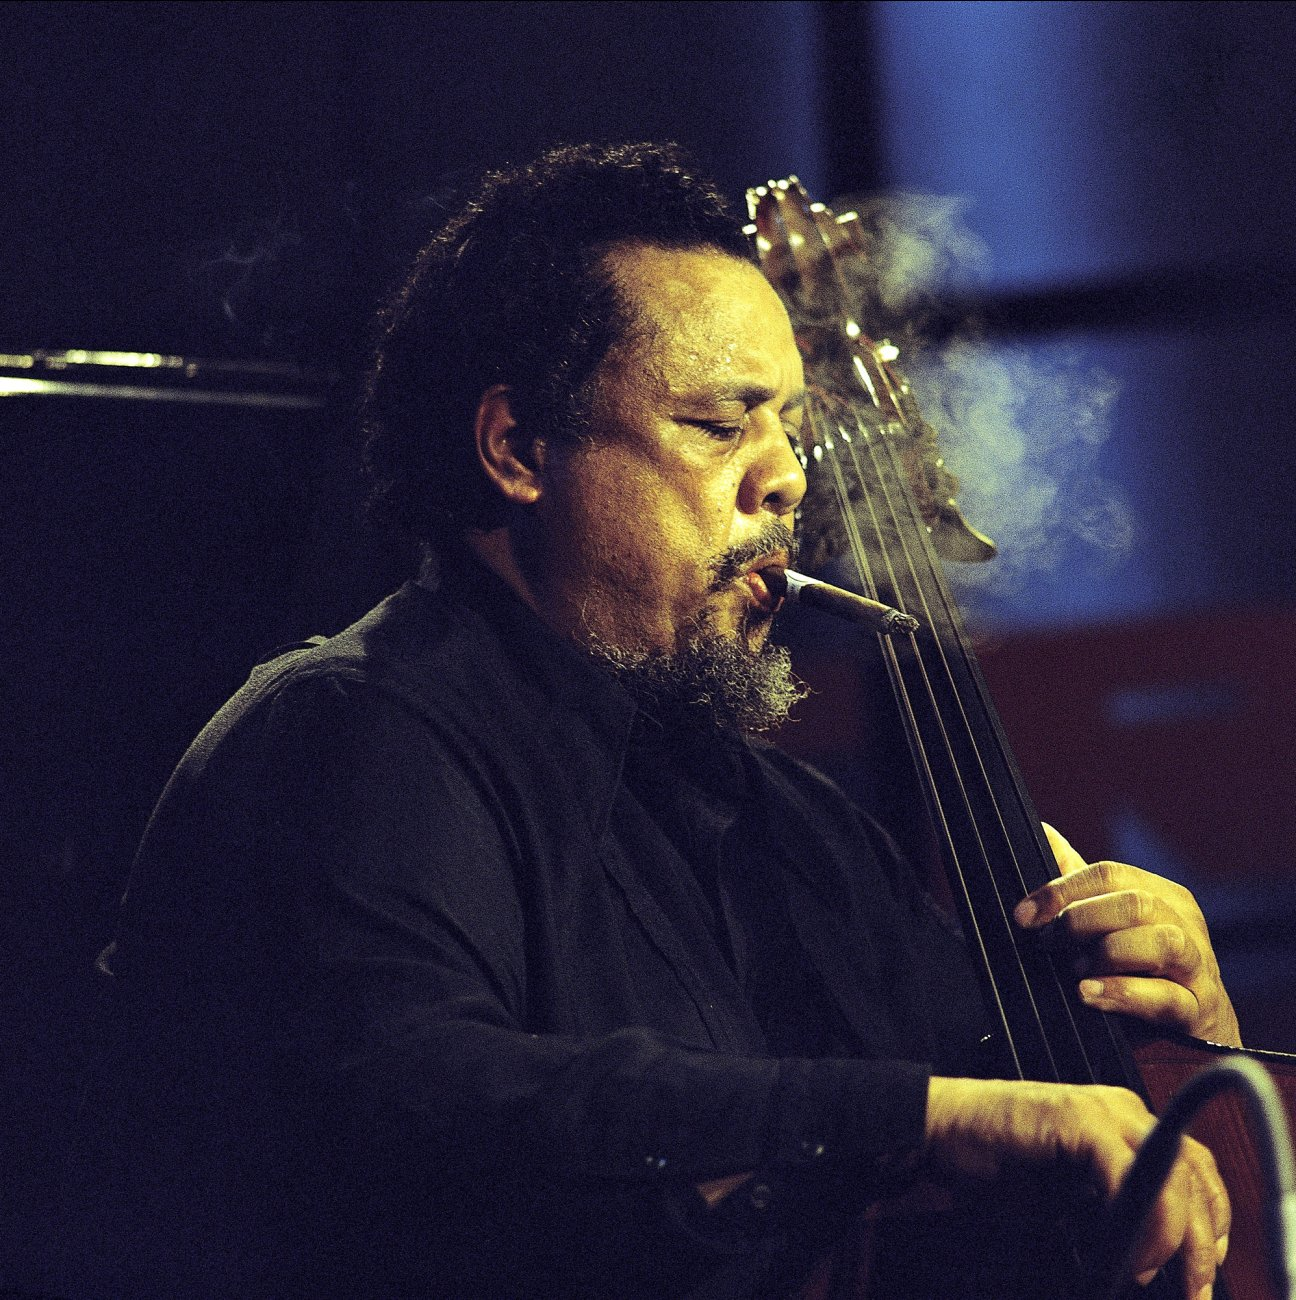
\includegraphics[width=0.5\textwidth]{report-2/fig/charles-mingus-1975.jpg}
    \caption{Charles Mingus}
    \label{fig:mingus_photo}
\end{figure}

Jazz improvisation is a good candidate for music generation, because its structure has limited need of long term memory: unlike other kinds of compositions, a jazz musician is unlikely to repeat structures that s/he has improvised minutes before. This characteristic could mitigate the issue of long term memory, a typical problem for language modeling. However, the complex phrasing and rhythmic structures and the sudden harmonic changes that characterize this style of music might be challenging for the transformer when capturing the relationship between the notes. 

MINGUS combines the architecture implemented by \cite{ECMG} with transformer models. An important difference between language and music is rhythm, which requires appropriate representation in the model. MINGUS attempts to solve this problem by treating the note duration as a separate feature, using a separate transformer model. Moreover, most of the models previously used for this task are not able to capture the entirety of the components which define a musical performance such as instrument timbre and interaction between musicians; these elements are especially important for improvisational music styles such as jazz, in which the interaction between different instruments is a fundamental component. MINGUS architecture will attempt to solve this problem conditioning each input on other musical features, such the harmonic structure, instrument and rhythm, however this feature has not yet been implemented. 

The purpose of this experiment is to explore the capability of the transformer to model and generate realistic melodic lines in the style of a jazz improvisation. It is also an opportunity to compare the performances of RNN-based models and transformers on musical data. 
Even though MINGUS has been trained specifically for music modeling and generation, its basic architecture could be easily modified to suite a number of other tasks such as score music classification, automatic harmonization, assisted composition, automatic music interpretation, conditional regression of musical features. 
The code used for the whole project can be found at \url{https://github.com/vincenzomadaghiele/MINGUS} (\cite{MINGUScode}).

\newpage

\section{State of the art} \label{sec:state of the art}
The generation of music can be approached by starting from audio or by starting from symbolic music representations. Both these approaches have their strengths and limitations. This experiment focuses on symbolic music generation, which is based on learning the dependencies between notes. Natural Language Processing (NLP) techniques, generally applied to language modeling, have been employed for this task. 

The state of the art deep learning models used for NLP are represented by two different network architectures, Recurrent Neureal Networks (RNNs) and Transformers, each with many possible variants. The most common variants of RNNs are LSTM and GRU, which are used to solve the problem of vanishing gradient, while the transformer structure, a newer technology, can be changed by omitting either the encoder or the decoder from the basic architecture. Both these technologies use the Sequence to Sequence (Seq2seq) approach, based on the encoder/decoder structure, in which the input sequence vector is encoded into a hidden vector, used to learn the dependencies between the data. 

\subsection{Data representation} \label{subsec: data representation}
Musical data can be represented symbolically with different levels of abstraction and precision. Many features could be extracted from purely musical data, such as pitch (frequency) and duration of the notes, relative position in the bar, harmonic structure, intensity (velocity), timbre. All of these factors contribute to the human perception of music and have been used to represent the musical data in the learning process. Another element of difference between the experiments in the literature is the granularity and the quality of the rhythmic representation. This aspect is explored by \cite{JazzGAN}, in which three different rhythmic representations are compared using the same network architecture. A common approach to represent duration in music is to treat it as a separate feature of a note which can be learned independently, as in \cite{ECMG}. An interesting alternative is provided in the work of \cite{seqAttn}, in which there is no notion of duration: a measure is split into 96 parts and a sustained note is represented by a sustain character '(s)', and the actual pitch character appears only when there is a change of pitch. All of these musical features can be used as conditions for training or as learnable elements. 

\subsection{Model architecture}
Many different architectures have been experimented in the literature for the specific task of music generation. The following summary focuses only on the models specifically studied for monophonic music generation. The main differences between these architectures are related to the structure of the model and the representation of the data. The simplest approach is jointly learning the dependencies between features in a unique RNN model. This approach has been experimented by \cite{C-RNN-GAN}, in which all the features are learned together by an adversarial network architecture combined with a deep RNN. The GAN structure has been used also by \cite{JazzGAN}, in which three separate GANs have been trained with different rhythmic encodings of the same dataset in order to evaluate the most effective one for this architecture. Another common approach is training separate models to learn different features of the data and then conditioning them on the other features. An example of this structure is the work of \cite{ACM}, in which two LSTM models are trained separately on pitch and duration of the notes in the melodies. The same architecture was used by B. Genchel \cite{ECMG} in their experiment Explicitly Conditioned Melody Generation (later referred to as ECMG in this report), in which they have trained the same architecture conditioning on different features (inter-conditioning between pitch and duration, chord, next chord and relative position in the bar) and compared the results. A different technique of data representation and sequence modeling has been adopted by \cite{seqAttn} (which will be referred to as SeqAttn later in this report), who have experimented with a modified LSTM attention unit. 
These last two architecture will be used as reference for this experiment's results, given that they represent good examples of the state of the art for this specific task using RNNs.

The aim of this experiment is comparing the result of these RNN based methods with a similar architecture based on a transformer module. The transformer model was first presented in \cite{AttnAllYouNeed}, and it has since proven very useful in different tasks of NLP. The transformer solves the problem of vanishing gradient which is typical of the RNN-based architectures. It is therefore possible to train transformer models on massive amounts of data and it has been used to achieve impressive results on generic tasks using big datasets. Examples of such networks are OpenAI's MuseNet (\cite{museNet}) and Magenta's Music transformer (\cite{MusicTransformer}), which both focus on the generation of polyphonic music.  

\subsection{Evaluation Methods}
Evaluating the performance of a generative task is an open problem, and in the literature many methods have been used to measure how realistic a music generation is. A common choice to measure the modeling capabilities of these methods are some classical machine learning metrics such as the loss function and the classification accuracy. These measures are related to the very nature of the sequence modeling problem, which is essentially a multi-class classification task, whose purpose is to predict the most probable class given the sequence of all the preceding classes. It could be argued that the purpose of this project and of the generation task more in general is not to obtain completely accurate prediction of the next token, so these metrics should not be considered to evaluate the quality of the model; nevertheless they are useful to make a comparison with the state of the art models. 

On a higher level, it is possible to use metrics which are commonly used to evaluate generative NLP tasks, such as perplexity and BLEU. Perplexity is closely related to the cross-entropy loss. It measures the amount of randomness in a model output on a given test set by evaluating the distribution of the probabilities on any output. The more a model is "undecided" (output probabilities are distributed among many values, so the amount of randomness is higher) the greater the perplexity. BLEU is a metric that has been developed specifically to evaluate the outcome of machine translation tasks (\cite{BLEU}). BLEU calculates the n-gram precision of a machine-translated sentence in comparison with a series of correct reference examples. Its application in music generation tasks is limited and it might be considered broadly as a measure of similarity between two corpus of music. It has been used in the ECMG paper and therefore it will be used in this experiment as a comparison, but its results are not a good indicator of how realistic a music generation can be. 
Other, more specifically music related, metrics have been proposed. These metrics are applied just to the outcome generated music. The concept behind these metrics is to measure how realistic a generated melody is by comparing it with the training corpus in specific musical terms. \cite{JazzGAN} propose a collection of metrics that can be used for this task, which include counting pitch repetitions, rhythmic variations and measuring harmonic consistency. \cite{MGEval} also propose the extraction of similar features. After feature extraction from both the training and the generated corpus the distributions of these features are compared by calculating the Kullback–Leibler divergence between them. The lower the divergence the more the two corpuses are similar.
Finally, many experiments of these kind are evaluated with qualitative human testing, by asking humans to distinguish the generated music from the original one, similarly to a Turing test. The higher the error rate of the humans in classification, the more realistic the generated music is.

\newpage
\section{Approach} \label{sec:approach}
The purpose of this experiment is to build a network that is specifically conceived to model complex music. Its architecture and data format allow to represent many different rhythmic configuration and duration values, and it is possible to train the model on different music styles without losing its effectiveness. 

\subsection{Datasets}\label{subsec:datasets}
MINGUS was trained on three different dataset to evaluate its adaptability to different styles of music and compare it with other state of the art models.

\subsubsection{Weimar Jazz DB}
The Weimar Jazz Database (\cite{Pfleiderer:2017:BOOK}) is a collection of transcriptions of jazz solos, composed of 453 improvisations on famous jazz standards by musicians playing multiple instruments. The dataset is composed of categorized midi files and complete with chords information. For this first phase of the experiment only the melody midi files have been used, but the chord information could be useful for model conditioning. After pre-processing this dataset is composed of 8019 melodic phrases (5667 for training, 767 for validation and 1585 for testing); the pitch dictionary is composed of 50 different pitch values and the duration dictionary is composed of 12 different duration values.
This dataset is by far the most complex among the three used and it provides a good example of how the MINGUS architecture is able to model complex music.

\subsubsection{FolkDB}
FolkDB is a dataset composed of 45848 scottish and irish folk songs, available in abc and midi format complete with chord transcriptions (\cite{folkDB}). After downloading the dataset in midi format some files have been excluded because of incompatibilities with the converting python library, resulting in 45825 midi files. 
This dataset has been chosen in order to compare the results to the ones obtained in the ECMG model. After pre-processing this dataset is composed of 229604 melodic phrases (160343 for training, 22932 for validation and 46329 for testing); the pitch dictionary is composed of 49 different pitch values and the duration dictionary is composed of 12 different duration values.
The music in this dataset is much simpler than the one in the Weimar Jazz DB.

\subsubsection{Nottingham DB}
The Nottighman database is a collection of 1034 folk songs in abc and midi format (\cite{NottinghamDB}). It has been chosen to compare the performance of MINGUS with those of the SeqAttn model on the same dataset. After pre-processing this dataset is composed of 5121 melodic phrases (3561 for training, 515 for validation and 1045 for testing); the pitch dictionary is composed of 31 different pitch values and the duration dictionary is composed of 11 different duration values. The music in this dataset is simpler than that of the Weimar Jazz DB, nevertheless its smaller dimensions could be useful to show how the dimension of the dataset influence the generation results.

\subsection{Data representation}
Before the data is used as input to the models it needs to be properly pre-processed. Many data formats are used in the literature for music generation. Among the most popular are the abc, musicXML and midi formats. All these formats store musical information with different degrees of precision. The midi format was chosen for this experiment because it allows to deal with timing with grater precision and most of the data was available in midi. The purpose of pre-processing is to transform the data from midi format to batched and model-ready data. 

\begin{figure}[!ht]
    \centering
    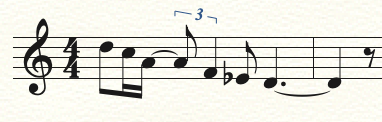
\includegraphics[width=0.5\textwidth]{report-2/fig/davis_oleo.png}
    \caption{Example melody, from Miles Davis improvisation on Oleo, Weimar Jazz DB} 
    \label{fig:Davis oleo}
\end{figure}

After reading the midi file each melody is split into a pitch and duration sequence, for example the melody in figure \ref{fig:Davis oleo} is split as follows:
\[P = [ 74, 72, 69, 65, 63, 62, R ] \]
\[D = [16th,\ 16th,\ 8th \ note \ triplet,\ dot \ 16th,\ 8th \ note \ triplet,\ dot \ quarter,\ 8th ]\]

$P$ is the pitch vector containing the midi number for each note and $D$ is a vector storing the duration of each note of the melody. The $R$ character in $P$ is the code for a rest. The duration value is extracted by sampling each measure of the midi file into 96 equally sized parts and assigning to each note the closest duration from a series of possible duration values chosen in advance; for example, the "quarter note" value is assigned to notes whose duration is closer to $measure \ duration \ [s] / 96 * 24$. In this specific case the choice to divide a measure into 96 equal parts allows for representation precision up to 8th note triplets and dotted 16th notes. By using a greater number of samples it would be possible to represent more precisely many different duration values. This method of time division ensures flexibility to different music styles which could require the use of more complex time divisions such as quituplets of septuplets. 

This procedure was applied to all the midi files in the dataset. After converting them into arrays, the frequency with which each unique pitch and duration value appears in the whole dataset has been calculated, and the values with very low frequency have been excluded from the data. 
The resulting arrays were then split into three subsets for training (70\%), validation (10\%) and testing (20\%). The next step is melody segmentation: language models are trained on batches of phrases with a maximum fixed length so also the training of MINGUS was done on batches of musical phrases. In order to divide each midi song into meaningful musical phrases the songs were split either when a long rest was encountered (long rests generally mark the end of a musical phrase) or when the maximum sequence length of 35 notes has been reached. The threshold for the long rest duration and the sequence length have been chosen experimentally by trial and error. The long rest durations are all of the durations that are greater than a quarter note triplet. By experimenting it has been found that a different choice of maximum duration, if not extreme, does not have much influence on the result, while the sequence length has a greater effect on the result. Another interesting observation is that the long rest must be included into the musical segment, otherwise the model will not learn the function of rests.
After the segmentation is complete all of the melodies that are shorter than 35 tokens are padded to that length with specific "pad" tokens. The 35-token sequences are then grouped into batches of 20 melodies for training and 10 melodies for validation and testing; they are then encoded and converted into tensors ready for network input. 

In order to obtain a bigger dataset some data augmentation techniques were applied to the input data. To augment the pitch data each pitch value was transposed a semitone up or down and the resulting transposed midi files were then added to the datasets. It is not possible to augment duration data, because modifying the duration of music makes the resulting melodies not realistic. 
Three datasets with different degrees of augmentation were generated by transposing each song respectively 1, 4 and 7 times. The model was trained on all of these datasets but no improvement in the results was found so the augmented datasets have not been used.

\subsection{Model Architecture}
MINGUS is structured as two parallel transformer encoder models with the same structure, one predicting pitch and another one predicting duration. This structure was chosen because it allows to capture the rhythmic variation with great precision, by allowing the model have a lot of different rhythmic codifications in the dictionary of the duration network. 
The basic structure of the Transformer model is described in \cite{AttnAllYouNeed}. Even tough the original transformer architecture is composed of encoder and a decoder modules, many popular language modeling networks use a variation of the transformer with only one of the two components. For example, OpenAI's GPT-2 (\cite{GPT2}) uses a structure made only of decoder modules, while google's BERT (\cite{devlin-etal-2019-bert}) is made only of encoders. 
The entire architecture used in this experiment is shown in figure \ref{fig:model architecture}. 

\begin{figure}[!ht]
    \centering
    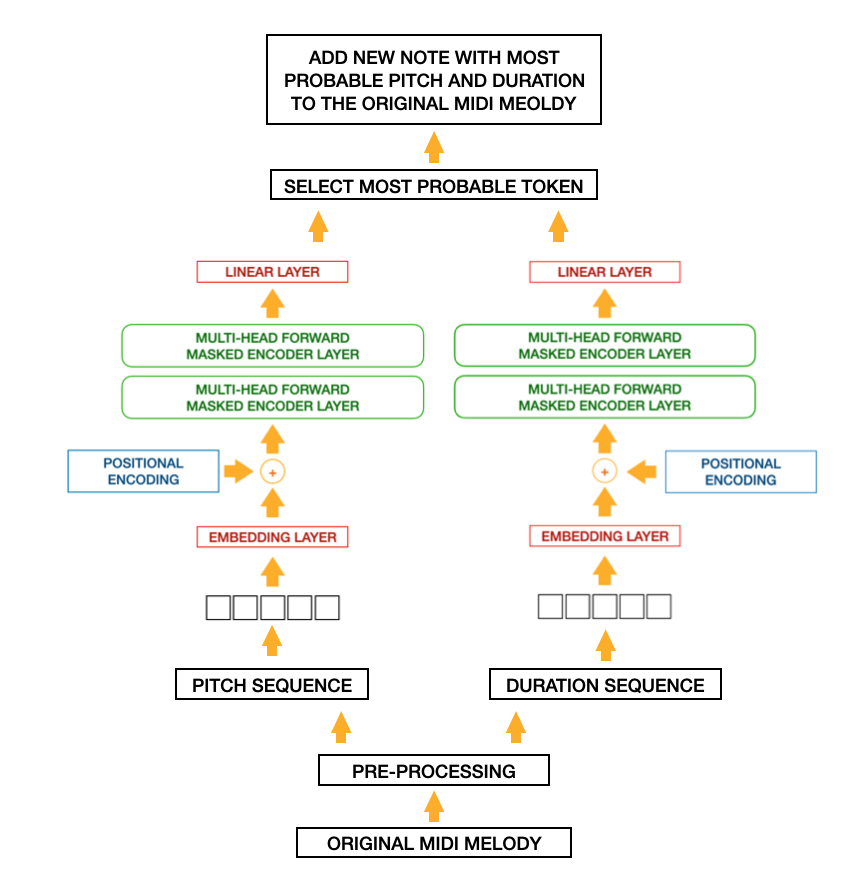
\includegraphics[width=0.7\textwidth]{report-2/fig/MINGUS_net_model.png}
    \caption{MINGUS model architecture 
    \label{fig:model architecture}}
\end{figure}

After pre-processing and batching the data goes through a linear embedding layer which represent each data point in a batch with a hidden 200-dimensional vector. The positional encoding is then applied to the embedded input in order to add the positional information into the data. The positional encoding is defined as:
\[ PE_{(pos,2i)} = sin(\frac{pos}{10000^{2i/d_{model}}})\]
\[ PE_{(pos,2i+1)} = cos(\frac{pos}{10000^{2i/d_{model}}})\]

This values are calculated for each entry in the embedded batch and added to it in order to store positional information. After this step the embedded batch goes into a two layer multi-head self-attention module, whose structure is described in figure \ref{fig:scaled dot}.

\begin{figure}[htbp]
    \centering
     \begin{subfigure}[b]{0.45\textwidth}
         \centering
         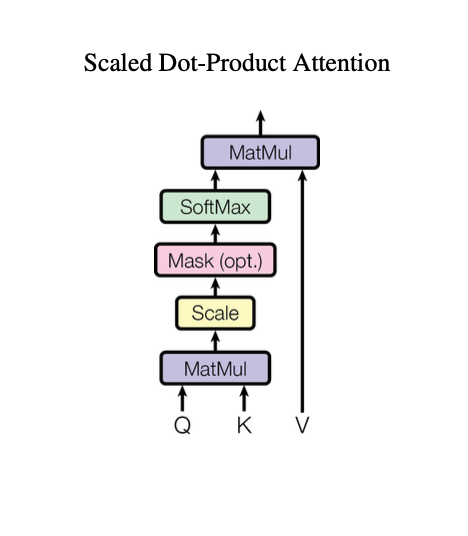
\includegraphics[width=\textwidth]{report-2/fig/Scaled dot product.png}
         \caption{Self-attention module}
         \label{fig:scaled dot}
     \end{subfigure}
     \hfill
     \begin{subfigure}[b]{0.45\textwidth}
         \centering
         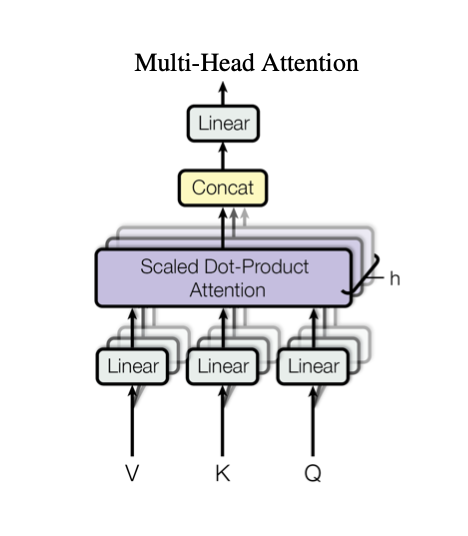
\includegraphics[width=\textwidth]{report-2/fig/multi-head attention.png}
         \caption{Multi-headed attention module}
         \label{fig:multi-head}
     \end{subfigure}
	\caption{}
	\label{fig:Attention module}
\end{figure}

The structure of the self-attention module can be divided into two parts, the first of which operates this transformation:

\[Attention(Q,K,V) = softmax(\frac{QK^T}{\sqrt{d_k}})V\]

Where $Q,K,V$, called Query, Key and Value, are replicas of the batched input after it goes through a linear layer. $Q$ and $K$ are then multiplied, scaled by $\sqrt{d_k}$ to avoid exploding gradient and then a softmax function is applied to the output. 
This step is different than the encoder module in the traditional Transformer architecture, because a square subsequent mask is applied to the batch in order to prevent the model to look at future tokens. The mask is applied after scaling by $d_k$ and before the softmax by multiplying all subsequent tokens by $- \infty$. Also a padding mask is applied in this step, in order to mask the padding tokens in the learning phase.
The matrix output of the softmax contains information about the mutual relationships between notes. The matrix is then multiplied by $V$; this operation returns the probabilities of the next note for each note in the processing batch. This vector is then added to the original batch and all is normalized; this step is called residual connection. It then goes through an point-wise feed forward network for further processing and a residual connection is operated again after the feed forward. As can be seen from figure \ref{fig:multi-head} this process is applied for $H$ times on different subset of the batched input in parallel, where $H$ is the number of attention heads that the self-attention module has. Both pitch and duration models in the MINGUS are composed of 2 attention heads and 2 layers of encoder. After the multi-head attention step the batched data goes through another linear layer which transforms the output from the embedding dimension to the token vocabulary dimension again, giving the probability for each token.

\subsection{Training, parameters tuning}
The network is trained with the task of predicting the next token given the tokens before in the sequence. Both pitch and duration models have been trained for 10 epochs by backpropagation of the Cross-Entropy loss function, using Stochastic Gradient Descent optimizer, with a dropout rate of 0.2. 
The generation is done by sampling the trained network given an input note sequence. The input melody is split into pitch and duration sequences and each sequence is given as input to the respective trained model. The output of the model are the probabilities for each token in the dictionary to be the next token. The most probable token is selected and added to the original sequence, which is then given back as input to the model. This process is repeated for as many times as the number of notes to be generated, which of course must be the same for pitch and duration. After generating the new sequences of pitch and duration separately they are added again into a midi file. 
It is possible to control the amount of randomness in the generation by choosing a temperature value between 0 and 1. This value is used to modify the output probability distribution of each token. The lower the temperature, the more random the next token selection will be. Adding randomness to the notes selection modifies the "creativity" of the model, and could lead to more interesting results from a musical perspective. Table \ref{tab:params} shows a summary of the training parameters used for both the pitch and the duration networks.

\begin{table}[htbp]
	\caption{MINGUS parameters for both pitch and duration network}
	\begin{center}
		\begin{tabular}{ p{5cm} p{2cm} }
             \hline
             \textbf{Parameter} &  
             \textbf{Value} \\
             \hline
             \hline
             Sequence Length & 35 \\
             Training batch size & 20 \\
             Validation batch size & 10 \\
             Testing batch size & 10 \\
             Epochs & 10 \\
             Hidden size & 200 \\
             Encoder layers & 2 \\
             Attention heads & 2 \\
             Dropout & 0.2 \\
             Epochs & 10 \\
             \hline
    \end{tabular}
	\label{tab:params}
	\end{center}
\end{table}

\newpage

\section{Results} \label{sec:results}
This section shows the results of MINGUS on various metrics in comparison with SeqAttn (\cite{seqAttn}) and ECMG (\cite{ECMG}). To obtain comparable results MINGUS has been trained on the three datasets described in section \ref{subsec:datasets}. It was possible to train the SeqAttn network with different datasets; the same is not true with ECMG, the reported metrics for this model are therefore the ones provided in their article and website for their unconditioned model. Moreover, when comparing the results obtained on folkDB by MINGUS and ECMG it should be taken into account that the modified version of folkDB used by ECMG was not available, the results are therefore not obtained on identical datasets.
When comparing perplexity and accuracy of MINGUS and SeqAttn the different representation of the duration must be taken into account. As explained in \ref{subsec: data representation}, in SeqAttn the duration of a note is represented by a sustain token "(s)" and this could influence the accuracy measurement, because the prediction of a sustain token is considered accurate even if the note that is being sustained is not correct; also the perplexity might be influeced due to the high frequency of sustain tokens that are easier to predict.

All the trainings have been performed on a macBook Pro, 8 GB RAM, 2.7 GHz Intel Core i5 dual-core CPU. The training times are reported in table \ref{tab:times}. The difference in training times is mainly due to the dimensions of the datasets.

\begin{table}[htbp]
	\caption{Training times on different datasets}
	\begin{center}
		\begin{tabular}{ p{2cm} p{2cm} p{2cm} }
		    \hline
             & \multicolumn{2}{c}{Training time [s]} \\
            \hline
            \textbf{Dataset} &  
            \textbf{Pitch} &
            \textbf{Duration} \\
            \hline
            \hline
            Weimar jazz & 345.58 & 297.89 \\
            Nottingham & 246.39 & 230.60 \\
            folkDB & 12674.96 & 40637.79 \\
            \hline
    \end{tabular}
	\label{tab:times}
	\end{center}
\end{table}

\subsection{Cross-Entropy loss and Perplexity}
As described in section \ref{sec:state of the art}, perplexity is a common metric for NLP tasks. It is strictly connected to the loss function, because it measures the level of uncertainty of the model by using the cross-entropy evaluated on test set. Perplexity is defined as:
\[Perplexity = e^{H(test)}\]
$H(test)$ is the cross-entropy function computed on the test set. The values of perplexity of both MINGUS and SeqAttn are collected in table \ref{tab:perplexity}. 

\begin{table}[htbp]
	\caption{Perplexity comparison between MINGUS and SeqAttn}
	\begin{center}
		\begin{tabular}{ p{2cm} p{2cm} p{2cm} p{2cm} }
             \hline
             Perplexity &  
             \multicolumn{2}{c}{\textbf{MINGUS}} & 
             \textbf{SeqAttn} \\
             \hline
             \textbf{Dataset} &  
             \textbf{pitch} & 
             \textbf{duration} & \\
             \hline
             \hline
             Weimar jazz & 13.2 & 2.3 & 6.29 \\
             Nottingham & 7.39 & 2.09 & 1.54 \\
             folkDB & 7.02 & 1.86 & - \\
             \hline
    \end{tabular}
	\label{tab:perplexity}
	\end{center}
\end{table}

The different rhythmic representation in SeqAttn and MINGUS make it difficult to compare the perplexity of the two models, however it is possible to compare how the perplexity of each model changes on the different datasets. The greatest perplexity value have been obtained for all models on the Weimar Jazz dataset, despite the fact that Nottingham DB has fewer data, proving that the complexity of the music is an important factor for language modeling tasks. The SeqAttn model has lower perplexity on the Nottingham DB, but the perplexity increases on the Weimar Jazz DB. The perplexity achieved by MINGUS on the duration does not change much as the complexity of the music increases, while instead the perplexity on the pitch model increases a lot because of the music complexity and of the greater dimension of the pitch dictionary.

\subsection{Accuracy and BLEU}
Accuracy measures how many times the model prediction for the next note is correct. This metric could be useful to have an overall view of the model performance but it does not guarantee a realistic musical generation. The accuracy values of MINGUS and SeqAttn on all datasets are reported in table \ref{tab:accuracy}.

\begin{table}[htbp]
	\caption{Accuracy comparison between MINGUS and SeqAttn}
	\begin{center}
		\begin{tabular}{ p{2.2cm} p{2cm} p{2cm} p{2cm}  }
             \hline
             Accuracy [\%] &  
             \multicolumn{2}{c}{\textbf{MINGUS}} & 
             \textbf{SeqAttn} \\
             \hline
             \textbf{Dataset} &  
             \textbf{pitch} & 
             \textbf{duration} & \\
             \hline
             \hline
             Weimar jazz & 13.92 & 58.62 & 47.26 \\
             Nottingham & 28.91 & 75.46 & 88.23 \\
             folkDB & 30.44 & 81.04 & - \\
             \hline
    \end{tabular}
	\label{tab:accuracy}
	\end{center}
\end{table}

It is difficult to compare the accuracy results because of the different note representation and of the division of pitch and duration models in MINGUS. The model achieves a very high accuracy on the duration prediction and lower accuracy in pitch predictions; this difference is due to the different size of vocabulary. Overall, considering the fact that a percentage of the accuracy of SeqAttn is due to prediction of sustain tokens, MINGUS accuracy seems to be comparable with that of SeqAttn.

BLEU is a popular metric used to measure the effectiveness of machine-translation models. In this application it has to be broadly intended as a measure of similarity between a generated song and 4 reference training samples. The BLEU values of MINGUS and ECMG are compared in table \ref{tab:BLEU}. 

\begin{table}[htbp]
	\caption{BLEU comparison between MINGUS and ECMG}
	\begin{center}
		\begin{tabular}{ p{2cm} p{2cm} p{2cm} p{2cm} p{2cm}  }
             \hline
             BLEU &  
             \multicolumn{2}{c}{\textbf{MINGUS}} & 
             \multicolumn{2}{c}{\textbf{ECMG}} \\
             \hline
             \textbf{Dataset} &  
             \textbf{pitch} & 
             \textbf{duration} &
             \textbf{pitch} & 
             \textbf{duration} \\
             \hline
             \hline
             Weimar jazz & 0.21 & 0.41 & - & - \\
             BebopDB & - & - & 0.098 & 0.875 \\
             folkDB & 0.24 & 0.07 & 0.26 & 0.87 \\
             \hline
    \end{tabular}
	\label{tab:BLEU}
	\end{center}
\end{table}

The BLEU score ranges from 0 to 1, and a high value indicates great similarity between the generated samples and the target corpus. The score obtained by MINGUS and ECMG on folkDB pitch models are really similar, instead the duration score is lower. This is a strange behaviour given that duration values should be easier to predict, but it is not concerning given that BLEU is not a very representative metric and that the duration model performs well on other, more representative metrics.

\subsection{MGEval}
MGEval is a collection of metrics specifically proposed by \cite{MGEval} for evaluation of generative music tasks. These metrics compute the degree of similarity between two corpus of midi files by extracting the distribution of each metric on the training corpus and on a corpus of generated musical sequences. The degree of similarity between the two corpus is then defined as the Kullback-Leibler divergence between the two distributions for each feature. MGEval also computes the overlap area between the two distributions. 
For each dataset the corpus of generated midi files is composed of 20 songs respectively. The generation for each song starts from the first 40 notes of an original song of the dataset; from those notes the model generates an amount of notes equal to the length of the original song of the training set. In some cases of very long songs it was necessary to stop the generation setting a maximum of 1000 notes to avoid very slow computation. The resulting distribution for MINGUS on the Weimar Jazz DB are shown in figure \ref{fig:MGEval}.

\begin{figure}[htbp]
    \centering
     \begin{subfigure}[b]{0.3\textwidth}
         \centering
         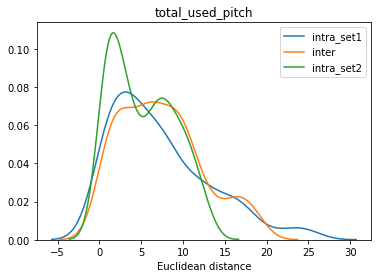
\includegraphics[width=\textwidth]{report-2/fig/TUP.png}
         \caption{Total used pitch}
         \label{fig:tup}
     \end{subfigure}
     \hfill
     \begin{subfigure}[b]{0.3\textwidth}
         \centering
         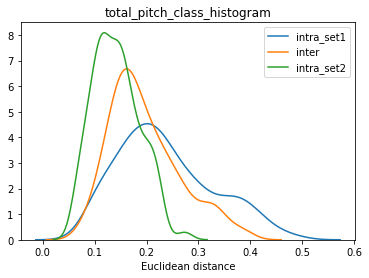
\includegraphics[width=\textwidth]{report-2/fig/TPCH.png}
         \caption{Total pitch class histogram}
         \label{fig:tpch}
     \end{subfigure}
     \begin{subfigure}[b]{0.32\textwidth}
         \centering
         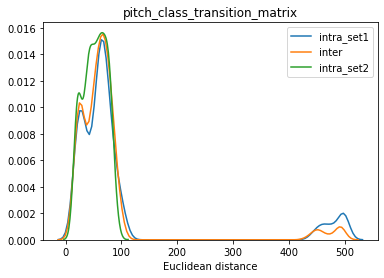
\includegraphics[width=\textwidth]{report-2/fig/PCTM.png}
         \caption{Pitch class transition matrix}
         \label{fig:pctm}
     \end{subfigure}
     \begin{subfigure}[b]{0.32\textwidth}
         \centering
         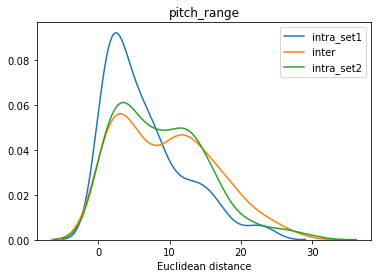
\includegraphics[width=\textwidth]{report-2/fig/PR.png}
         \caption{Pitch range}
         \label{fig:pr}
     \end{subfigure}
     \begin{subfigure}[b]{0.3\textwidth}
         \centering
         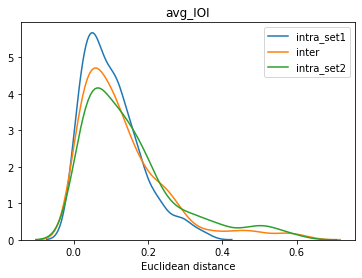
\includegraphics[width=\textwidth]{report-2/fig/IOI.png}
         \caption{Avg IOI}
         \label{fig:ioi}
     \end{subfigure}
	\caption{MGEval metrics distribution on MINGUS results on Weimar jazz DB}
	\label{fig:MGEval}
\end{figure}

In figure \ref{fig:MGEval} the blue lines are the distributions computed in the training set composed of the original data, while the green line show the distribution of the same metric computed on the generated midi files. The more the two curves look alike, the more the metrics computed on the two corpus are similar. The orange line shows the metric computed on a union of both datasets. 

The metrics considered in this experiment are total used pitch, total pitch class histogram, pitch class transition matrix, pitch range and avg IOI. Other metrics are provided by MGEval but they have not been used in this experiment because of incompatibility between the MGEval code and the dataset midi tracks. Total used pitch is defined as a scalar counting the total number of unique pitches (octave-dependent) used. The total pitch class histogram is a histogram of the number of octave-independent pitch classes used in a sample, a vector of size 12. The pitch class transition matrix is a histogram-like representation computed by counting the pitch transitions for each (ordered) pair of pitch classes (octave is not considered). The pitch range is calculated by subtraction of the highest and lowest used pitch in semitones, the output is a scalar for each sample. Avg IOI is a scalar value, the average distance between note beginnings. 

Table \ref{tab:MGEval folkDB} collects the results of obtained by these MGEval metrics on MINGUS and ECMG models trained on folkDB.

\begin{table}[htbp]
	\caption{MGEval comparison between MINGUS and ECMG on folkDB}
	\begin{center}
		\begin{tabular}{ p{5cm} p{1.5cm} p{2.2cm} p{1.5cm} p{2.2cm}  }
            \hline
            MGEval & 
            \multicolumn{2}{c}{\textbf{MINGUS}} & 
            \multicolumn{2}{c}{\textbf{ECMG}} \\
            \hline
            \textbf{Measure} &  
            \textbf{KL div} & 
            \textbf{overlap area} &
            \textbf{KL div} & 
            \textbf{overlap area} \\
            \hline
            \hline
            total used pitch & 0.011 & 0.770 & 0.025 & 0.888 \\
            total pitch class histogram & 0.069 & 0.707 & 0.242 & 0.686 \\
            pitch class transition matrix & 0.137 & 0.813 & 0.026 & 0.714 \\
            pitch range & 0.033 & 0.757 & 0.019 & 0.849 \\
            avg IOI & 0.074 & 0.765 & 0.533 & 0.480 \\
            \hline
    \end{tabular}
	\label{tab:MGEval folkDB}
	\end{center}
\end{table}

MINGUS performs better on some metrics, such as total used pitch, total pitch class histogram and avg IOI, while ECMG performs better on pitch class transition matrix and slightly better on pitch range. The most interesting comparison is probably between the pitch class transition matrix. The difference difference between the two values means that the transitions between different pitch classes have been learned better by the ECMG model. The two most significant metrics in which MINGUS does better than ECMG are instead the total pitch class histogram and the avg IOI. The result obtained on the pitch class histogram means that the choice of notes in absolute terms operated by MINGUS is more similar to the one in the training set. The result of avg IOI instead gives information about the rhythmic distribution of notes. The better result obtained by MINGUS in this metric means that it mimics the choice of the training set regarding duration values better than the ECMG model.
Overall, by this comparison it seems that the RNN model proposed in ECMG captures better the short-term sequential component of the data, measured in the pitch class transition matrix, but the transformer is able to do a much better modeling of the general distribution of the pitch classes in the training dataset and mimics it when generating new notes. 

The result obtained by MINGUS on the other two datasets on these MGEval metrics are collected in table \ref{tab:MGEval jazz, nottingham}.

\begin{table}[htbp]
	\caption{MGEval comparison between Weimar jazz DB and Nottingham DB on MINGUS generations}
	\begin{center}
		\begin{tabular}{ p{5cm} p{1.5cm} p{2.2cm} p{1.5cm} p{2.2cm}  }
            \hline
            MGEval & 
            \multicolumn{2}{c}{\textbf{Weimar jazz DB}} & 
            \multicolumn{2}{c}{\textbf{Nottingham DB}} \\
            \hline
            \textbf{Measure} &  
            \textbf{KL div} & 
            \textbf{overlap area} &
            \textbf{KL div} & 
            \textbf{overlap area} \\
            \hline
            \hline
            total used pitch & 0.068 & 0.408 & 0.045 & 0.824 \\
            total pitch class histogram & 0.059 & 0.280 & 0.151 & 0.718 \\
            pitch class transition matrix & 0.186 & 0.413 & 0.577 & 0.711 \\
            pitch range & 0.045 & 0.48 & 0.057 & 0.786 \\
            avg IOI & 0.004 & 0.778 & 0.008 & 0.916 \\
            \hline
    \end{tabular}
	\label{tab:MGEval jazz, nottingham}
	\end{center}
\end{table}

These results on different datasets show a coherence between the metrics results. It seems that all the generations by MINGUS perform similarly on MGEval even though the dataset changes. This confirms that these metrics reflect the strengths and the weaknesses of the transformer model for this task rather than the properties of the different datasets. The worse performance on Nottigham DB are probably due to the fact that it is a smaller dataset. Overall, comparing the results obtained on the Weimar Jazz DB and folkDB it is possible to notice that even though the music in the Weimar Jazz DB is much more complex and diverse MINGUS's performance is consistent and the results on these metrics are not so different. The same cannot be said of the performance difference of ECMG between folkDB and BebopDB (cited in their paper); in their case the metrics are quite different and the results on BebopDB fall. However this comparison is not explored more in depth because BebopDB is not available and it was not possible to train MINGUS on it.

\subsection{Musical analysis of the generations}
The generations are fairly realistic but, as can be seen by analyzing the score more in depth, the model still lacks of a long-term coherence among the musical phrases. Moreover, also on a phrase-level inspection the generated music struggles to present a completely realistic structure. This can be seen by comparing a phrase of an original improvisation in the Weimar jazz database to a generated phrase over the same song. This difference is represented quite clearly in figure \ref{fig:mr PC}.

\begin{figure}[htbp]
    \centering
     \begin{subfigure}[b]{0.9\textwidth}
         \centering
         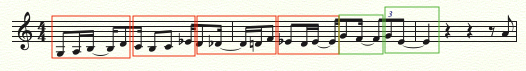
\includegraphics[width=\textwidth]{report-2/fig/MrPC original.png}
         \caption{Original improvised phrase}
         \label{fig:mrPc original}
     \end{subfigure}
     \hfill
     \begin{subfigure}[b]{0.9\textwidth}
         \centering
         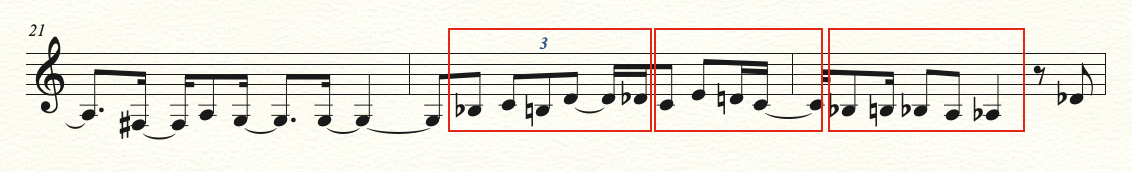
\includegraphics[width=\textwidth]{report-2/fig/MrPC gen.png}
         \caption{MINGUS generated phrase}
         \label{fig:mr PC generated}
     \end{subfigure}
	\caption{Comparison of original and generated musical phrases on Mr PC by John Coltrane, part of the Weimar Jazz DB}
	\label{fig:mr PC}
\end{figure}

Figure \ref{fig:mrPc original} shows a phrase from the original improvisation of John Coltrane on his song Mr P.C., while figure \ref{fig:mr PC generated} represents a phrase generated by MINGUS on the same song, which is a good example of how the model behaves when generating music.
By analyzing the original melody it is possible to identify its underlying structure by dividing it into smaller groups of notes, called motifs, which have similar melodic and rhythmic structure. In the first example many subsequent variations of the same motif, indicated in red, are played one after the other in an ascending fashion, while the last motif of the phrase, indicated in green, is repeated twice with a small closing variation. In the generated phrase, instead, it is only possible to spot a similar behaviour on the local level, but the relationship between subsequent motifs is not as well defined as in real improvised melodies and it is not coherent as the melody goes on. 

This distinction is even more evident comparing how different phrases are connected. While in the original improvisations it is generally possible to identify the call and response structure between musical periods, it is not possible to do it between the generated periods. This was expected because the model is trained on phrase-level sequences of maximum 35 notes. This also explains why, while in the original jazz improvisation there is a clear distinction between the start and the end of a phrase, in the music generated by MINGUS it is not clear when a musical phrase ends and another one begins. 
Another interesting aspect of the generation model can be evaluated by rhythmic analysis of the melodies; the two phrases in the figure have similar rhythmic structure, and the rhythmic structure of the motifs highlighted in red in the generated melody is more coherent than the pitch structure, because it repeats exactly. 
In general it is possible to observe that the rhythmic structure of the melodies is more realistic than the pitch structure. This confirms the results obtained by the measures in the previous sections, which all highlight the better performance of the duration model.

\newpage
\section{Conclusions} \label{sec:conclusion}
MINGUS provides a transformer architecture specifically designed to handle complex music. The model was experimented on three different popular datasets and evaluated using different high and low level metrics. Its performances have been satisfactory on most metrics, reaching the level of state of the art models. Comparing its results on datasets of different complexity and dimension it was possible to see that the model is capable of producing state of the art music generations for all of the different styles of music. 

One of the main limitations of this experiment is that the very nature of jazz music is not related to its symbolic representation as much as other forms of music, because of its inherent improvisational nature. A jazz improvisation has to be interpreted in the harmonic and rhythmic context of what the other instruments are playing, which can be very different from the harmonic structure of the original tune. Analyzing the transcription of a jazz solo based only on the chords of the standard can be quite limiting because it takes the relationship between instruments and musicians out of the symbolic representation. 
Many considerations could be made regarding the differences between the thought process of the jazz soloist and a classical composer, and how this affects the symbolic representation of the music and therefore the learning possibilities of a machine learning model. 
These kind of considerations find an application in the choice of conditional models: conditioning a jazz melody on chords might or might not be a good choice depending on the style of jazz, and for some songs it might be much more useful to condition the melody on the bass line or the rhythmic structures played by the drums. Unfortunately it is very difficult to find datasets that contain all of these information and it is therefore necessary to operate a generalization and omit a lot of the context of each jazz solo from its hidden representation in the model. Nevertheless, having the possibility to condition the generation of a melodic line on what all the other instruments are playing would be a very interesting experiment. 
Other limitations are related to the fact that MINGUS is not capable to correctly model the relationship between musical phrases and to achieve a long term coherence. This aspect is still an open problem for more general NLP tasks, and it could be interesting to apply some of the techniques that are being used to overcome it to this particular model.

On a personal level, this project has been challenging for many reasons, but it has been really satisfying too. I learned to research topics in state of the art scientific articles, I have learned how to build a transformer model and how to deal with deep learning problems more in general. Probably the biggest lesson that I have learned has been that simple tweaks such as adding a pad masking to the data can make a significant difference on the results in deep learning models, and that parameter tuning is really important for a well functioning model. 

This project could be expanded in many direction. Surely, it has to be completed by conditioning the model on chords and other musical features and tested again with respect to other conditional models; another interesting direction could be expanding the model in order to achieve long term phrase level coherence. A conditional model could then be trained to interact with a live musician, implementing an interface for it to interpret live inputs and reacting consequently. Moreover, the architecture of MINGUS could be expanded for tasks different from music generation, such as style classification, automatic harmonization and regression of other musical parameters.

\newpage
%%%%%%%%%%%%%%%%%%%%%%%%%%%%%%%%%%%%%%%%%%%%%%%%%%%%%%%%%%%%%%%%%

\bibliography{mybibfile}
\end{document}